\documentclass{jfp1}

%%%%%%%%%%%%%%%%%%%%%%%%%%%%%%%%%%%%%%%%%%%%%%%%%%%%%%%%%%%%
% Global switches
%%%%%%%%%%%%%%%%%%%%%%%%%%%%%%%%%%%%%%%%%%%%%%%%%%%%%%%%%%%%

% Turn on to include todos and comments.  These are intended for stuff
% we need to do or discussions that may influence the text of the
% paper itself.
\newif\ifcomments\commentstrue

% Turn on to include commentary. This is intended for stuff we want to
% remember/write down but do not intend to include in the paper.
\newif\ifcommentary\commentarytrue

%%%%%%%%%%%%%%%%%%%%%%%%%%%%%%%%%%%%%%%%%%%%%%%%%%%%%%%%%%%%
% Packages
%%%%%%%%%%%%%%%%%%%%%%%%%%%%%%%%%%%%%%%%%%%%%%%%%%%%%%%%%%%%

\usepackage[T1]{fontenc}
\usepackage[utf8]{inputenc}
\usepackage[override]{cmtt}
\usepackage{hyperref}
\usepackage{mdframed}
\usepackage{comment}

\usepackage{graphicx}
\graphicspath{{images/}}

\usepackage{latex/agda}
% for grabbing pieces of Agda from a different file, so that latex and
% Agda don't have to mix too much.
\usepackage{catchfilebetweentags}

\usepackage[backend=pgf, outputdir=diagrams]{diagrams-latex}
\usepackage{pgf}

%%%%%%%%%%%%%%%%%%%%%%%%%%%%%%%%%%%%%%%%%%%%%%%%%%%%%%%%%%%%
% Unicode
%%%%%%%%%%%%%%%%%%%%%%%%%%%%%%%%%%%%%%%%%%%%%%%%%%%%%%%%%%%%

% See https://agda.readthedocs.io/en/v2.6.0.1/tools/generating-latex.html

\usepackage{newunicodechar}
\newunicodechar{∀}{\ensuremath{\forall}}
\newunicodechar{ℓ}{\ensuremath{\ell}}
\newunicodechar{→}{\ensuremath{\to}}
\newunicodechar{λ}{\ensuremath{\lambda}}
\newunicodechar{ℕ}{\ensuremath{\mathbb{N}}}
\newunicodechar{∘}{\ensuremath{\circ}}

%%%%%%%%%%%%%%%%%%%%%%%%%%%%%%%%%%%%%%%%%%%%%%%%%%%%%%%%%%%%
% Typesetting
%%%%%%%%%%%%%%%%%%%%%%%%%%%%%%%%%%%%%%%%%%%%%%%%%%%%%%%%%%%%

\newcommand{\term}[1]{\emph{#1}}

%%%%%%%%%%%%%%%%%%%%%%%%%%%%%%%%%%%%%%%%%%%%%%%%%%%%%%%%%%%%
%% Comments
%%%%%%%%%%%%%%%%%%%%%%%%%%%%%%%%%%%%%%%%%%%%%%%%%%%%%%%%%%%%

\ifcomments
\newcommand{\authornote}[3]{\textcolor{#1}{[#3 ---#2]}}
\newcommand{\todo}[1]{\textcolor{red}{[TODO: #1]}}
\else
\newcommand{\authornote}[3]{}
\newcommand{\todo}[1]{}
\fi

\newcommand{\bay}[1]{\authornote{blue}{BAY}{#1}}
\newcommand{\jc}[1]{\authornote{green}{JC}{#1}}  % pick whatever
                                                 % color/initials you want

\ifcommentary
  \newmdenv[skipabove=1em, skipbelow=1em, innermargin=1.5em, outermargin=1.5em, backgroundcolor=black!8, linecolor=black!10]{commentary}
\else
  \excludecomment{commentary}
\fi

%%%%%%%%%%%%%%%%%%%%%%%%%%%%%%%%%%%%%%%%%%%%%%%%%%%%%%%%%%%%
% Front matter
%%%%%%%%%%%%%%%%%%%%%%%%%%%%%%%%%%%%%%%%%%%%%%%%%%%%%%%%%%%%

\title{Memory Models via Species: The Paper}
\subtitle{Or: You Could Have Invented Species, If You Happened To Think
  About It In This Very Specific Way}
\author[J. Carette and B. A. Yorgey]{JACQUES CARETTE\\
  McMaster University, Ontario, Canada \\
  \email{carette@mcmaster.ca}
  \and BRENT A. YORGEY\\
  Hendrix College, Arkansas, USA\\
  \email{yorgey@hendrix.edu}}

%%%%%%%%%%%%%%%%%%%%%%%%%%%%%%%%%%%%%%%%%%%%%%%%%%%%%%%%%%%%

\begin{document}

\commentary{I (JC) don't think we should put Species, the word,
in the title at all. I have no problems with using the current
title as the working title, but we'll see how things develop.}

\maketitle

What is a \term{memory}?  We will start by taking the abstract
position that \emph{a memory is a store of values}, that is,
an abstract container where values can be stored and later retrieved.

\begin{commentary}
  This used to say ``a collection of locations where
values can be stored and later retrieved'', but that is, in some
ways, double indirection -- at least it will be as soon as labels
are introduced.  I'm not so sure about the word ``container'', but
that can be figured out later.
\end{commentary}

\begin{figure}[htp]
  \centering
  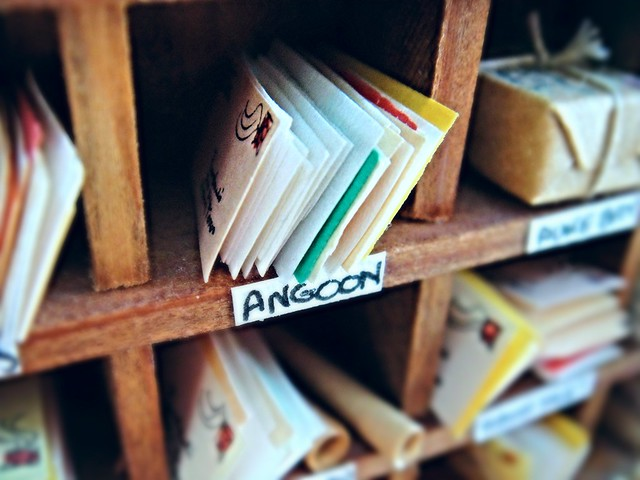
\includegraphics[width=0.5\textwidth]{mailboxes.jpg}
  \caption{A memory with labelled locations. Photo by JLS Photography.\protect\footnotemark}
  \label{fig:mailboxes}
\end{figure}
\footnotetext{\url{https://www.flickr.com/photos/akgypsy37/8690531067/}, CC BY-NC-ND 2.0.}

\begin{commentary}
  The intent of the picture is to show a very physical
notion of ``labelled memory'', where the labels are quite
visible, and there are physical things ``stored'' at the address
indicated by the label.
\end{commentary}

What sort of structure does a memory need to have to make this
possible?  If there are to be many values stored in memory, and
we want to somehow retrieve a particular one, how can we do that?
In order to retrieve values, there must be a way to refer to where
they are stored, so we suppose that we possess a \emph{label}
for that purpose. Then a \term{memory}
is just a way to associate values to labels.

\jc{The above is now a bit woolly. It's still better than
using location, but it can surely be made crisper}

\todo{Remove the term ``location''! No double indirection!}

Here is one model: a function from labels to values.  Lookup is just evaluation. 
However, there are many other models, and so we don't want to commit
to just one model so early.

\begin{commentary}
  There is a subtle issue with the next paragraph: in the picture it
  is actually the \emph{locations} which are in a 2D grid; the
  \emph{labels} themselves (presumably) do not reflect this structure.
  Ultimately, the concept of ``locations'' is there as a conceptual
  aid, but is not directly reflected in our framework.  In the
  physical world, one could take the physical coordinates of locations
  (relative to some reference) as a set of labels, and then going from
  (what we would usually think of as) a ``label'' to physical
  coordinates is accomplished by a final relabelling operation, where
  the ``relabelling'' isomorphism is actually (in one direction) an
  algorithm for doing some sort of physical search.  For example, if
  you know the call number (one set of labels) of a book in a library,
  the facts that (1) the call numbers have a total ordering and (2)
  the books are arranged in physical space in a particular way
  according to the ordering---i.e. there is an \emph{order-preserving
    isomorphism} between call numbers and physical locations---means
  that you can perform something like a binary search in physical
  space to find the physical location (another set of labels) of the
  book you want.  (To compute the other direction of the isomorphism,
  of course, you just look at the call number printed on the spine of
  a book---though it's interesting/notable that in the case of a
  library it's actually the \emph{values} (i.e. books) that are
  labelled with call numbers rather than the locations themselves.
  Declining to label the locations with call numbers is an
  optimization that allows for easier compaction/garbage
  collection\dots) It's interesting that to carry out one direction of
  the isomorphism (call number -> physical location) requires
  repeatedly running it in the opposite direction (pick a physical
  location, find the call number of the book there, and compare to
  your chosen call number to decide which direction to go next).

  In RAM, of course, the last relabelling to convert a physical
  address into a physical location doesn't use search, but rather a
  circuit which selects a physical location based on the bit pattern
  used to encode the address.  This relabelling is also
  order-preserving in a certain sense, though that's only because it
  leads to a nice/efficient/concise circuit; there's no a priori
  reason we couldn't build a circuit which maps consecutive addresses
  to arbitrary non-consecutive physical locations.
\end{commentary}

For now, we don't assume that labels have any special structure
(though some particular sets of labels might).  For example, the
locations in Figure~\ref{fig:mailboxes} are evidently arranged in a 2D
grid, but this is a special case.  In the abstract, it may be
helpful to imagine a memory as a ``soup'' of locations, labelled by
arbitrary names.  As an illustration, Figure~\ref{fig:soup} shows a
memory with only three locations. The locations are not arranged in
any particular relation to one another; moreover, the labels have been
chosen to emphasize that the set of labels can be entirely arbitrary,
without any sort of inherent structure.  The labels may or may not
have decidable equality, may or may not be concretely representable as
sequences of bits, and so on.

\begin{figure}
  \centering
  \begin{diagram}[width=150]
  drawLocation :: Diagram B -> Diagram B -> Diagram B
  drawLocation lab val = vsep 0.2 [val <> roundedRect 1 1 0.1, lab]

  locs cow = zipWith drawLocation
    [ circle 0.2 # fc blue # lw none
    , text "$\\alpha$" # fontSizeL 0.5 <> phantom (square 0.5 :: D V2 Double)
    , image cow # sized (dims (1 ^& 1))
    ]
    (map (fontSizeL 0.8 . text . show) [2, 7, 5])

  cs =
    [ origin
    , 3 ^& (-2)
    , 4 ^& 1
    ]

  dia :: IO (Diagram B)
  dia = do
    Right cow <- loadImageEmb ("images/cow.png")
    return $ mconcat (zipWith moveTo cs (locs cow))  -- $
  \end{diagram}
  \caption{A ``soup'' of labelled locations storing integer values}
  \label{fig:soup}
\end{figure}

Along the same lines, although we will use Agda \todo{cite} as a
concrete metalogic in which to express our ideas, we make no
particular commitments to the specific metalogic used and what
features it may or may not have available.  For example, Agda has many
built-in type formers (sums, products, \emph{etc.}) which allow one to
construct new types out of existing ones, but we will not take such
type formers for granted.  In general, the name of the game is to add
structure in a gradual, carefully controlled manner, so as to discover
the minimum amount of structure necessary to model various phenomena.

\begin{commentary}
  In fact what we are committing to up front is simply a category
  where objects are types, with some notion of morphisms between
  types.
\end{commentary}

\subsection{Relabelling}
\label{sec:relabelling}

The first nontrivial operation we require memories to have is
\emph{relabelling}: it should be possible to change the labels on a
memory by specifying a new set of labels along with a specification of
how the new labels map onto the old.

\ExecuteMetaData[latex/models.tex]{relabel}

The first thing to notice is that $\AgdaFunction{Memory}$ is
\emph{contravariant} in $\AgdaBound{L}$. \todo{explain}.

Notice also that the provided relabelling function need not be a
bijection.

\begin{itemize}
\item The relabelling function might not be surjective, that is, some
  of the old labels might be left out. This allows us to model
  deleting or ``freeing'' memory that is no longer needed.
\item Likewise, the relabelling function might not be injective, that
  is, multiple new labels may map to the same old label.  This allows
  us to model aliasing.

  ``bags for free''.

  ``aliasing'' is a loaded term!  Implies mutability, i.e. assign
  operation.  Leave that until later.
\end{itemize}

\todo{motivate relabel: one model is to actually change the labels.
  Another is to just store a function off to the side.  e.g. array
  libraries, virtual memory}

\todo{draw a picture of relabelling.}

Note that a $\AgdaFunction{Memory}$ must be a \emph{total} function,
that is, every label corresponds to some value.  If we wish to model
memories where some labels do not correspond to a stored value, we can
simply use a type $V$ of values with a distinguished ``empty'' value.
\todo{Actually there are other choices too!  e.g. get rid of labels
  entirely.  This is why we're going to wait.}

\begin{commentary}
  relabel is still useful if $L' = L$.  e.g. Copying garbage collection.
\end{commentary}

\todo{eventual motivation: represent data structures!  So we need some
structure on labels (?)  Next up: disjoint union.  Related to malloc:
what to do if someone hands you some new labels.  Look at haskell/src/Data/Storage.hs}

\begin{commentary}
  Models with and without functoriality for values!  Might have to do
  something like co-Yoneda trick to make it functorial.
\end{commentary}

\bay{At some point in the future we will want to talk about label
  equality, but not yet.  Don't you need decidable equality at the
  point where you want a ``set'' operation (i.e. an operation that
  takes a memory, a label, and a (new) value, and sets the value at
  the given location, returning a new updated memory)?}

\subsection{Label equality}
\label{sec:label-equality}

As an example, take $L = \mathbb{R}$ to be the set of real numbers.
A ``memory'' with this set of labels is thus an assignment of a value
to every point on the real line.

Although this is well-defined, it is hard to imagine how one could
actually do anything with such a memory.  The problem is that
\bay{how to say exactly what the problem is?  Is this actually a good
  example?  It seems like it may actually be combining several
  problems (uncountable number of elements; uncomputable elements; no
  decidable equality\dots)}

We will thus usually want to limit ourselves to label sets $L$ which
come with a decidable equivalence relation, and require that the
mapping from labels to values respects this equivalence (that is,
equivalent labels are never mapped to different values).

\bay{What Agda code should go along with this?}


\begin{commentary}
  Simplest data structure: singleton-indexed.  Next: two-element-set
  indexed, i.e. a pair.  Note it is not necessarily an ORDERED pair!
  Talk about relabelling, functoriality, groupoids...

  Distinction between single structures and *collections* of
  structures (aka species aka data types).

  'assign' operation requires decidable equality?

  Laws for lookup/assign?  Interacts with what kind of relabelling is
  allowed.

\end{commentary}

\end{document}
